\section{问题三的建模与求解}

\subsection{问题分析}

问题三提出了最严格的约束：同时指定任意的镜面图案 $M^*$ 和纸面图案 $P^*$，仅靠艺术加工，能否设计出两者均有意义的作品？这一问题的本质是一个双目标逆问题——实际纸面图案 $I_P$ 需要同时满足两个相互竞争的目标：（1）$I_P$ 在视觉上接近指定的纸面目标 $P^*$；（2）$I_P$ 经正向映射后的镜面图案 $F(I_P)$ 接近指定的镜面目标 $M^*$。由于正向映射 $F$ 是一个非线性几何变换，两个目标之间存在本质的矛盾——除非 $P^*$ 恰好等于 $f^{-1}(M^*)$（即纸面目标恰好是镜面目标的逆映射），否则不可能同时完美满足两个目标。因此，问题三的核心在于量化这种矛盾的程度，并找到使两个目标达到最佳折中的条件。

\subsection{双目标优化模型}

同时指定纸面目标图案 $P^*$ 和镜面目标图案 $M^*$，寻找实际纸面图案 $I_P$ 使两者误差最小：

$$
\min_{I_P} \; \mathcal{L}(I_P) = \lambda_1 \|I_P - P^*\|_F^2 + \lambda_2 \|F(I_P) - M^*\|_F^2
$$

其中 $\|\cdot\|_F$ 为Frobenius范数（逐像素 $L^2$ 误差），$F$ 为正向映射算子，约束条件为 $I_P(x,y) \in [0,255]^3$。权重 $\lambda_1$ 和 $\lambda_2$ 控制两个目标的相对重要性，$\lambda_1 + \lambda_2 = 1$。

对目标函数求一阶变分，得到最优性必要条件：

$$
2\lambda_1 (I_P - P^*) + 2\lambda_2 F^T(F(I_P) - M^*) = 0
$$

其中 $F^T$ 为正向映射算子的伴随算子。从物理意义上理解，$F^T$ 将镜面空间中的误差信号"反向传播"到纸面空间，类似于神经网络中的反向传播机制。最优性条件表明，最优纸面图案 $I_P^*$ 是纸面目标 $P^*$ 和镜面目标逆映射 $f^{-1}(M^*)$ 的某种加权折中。

采用梯度下降法迭代求解：

$$
I_P^{(k+1)} = I_P^{(k)} - \eta \bigl[\lambda_1(I_P^{(k)} - P^*) + \lambda_2 F^T(F(I_P^{(k)}) - M^*)\bigr]
$$

初始值取 $I_P^{(0)} = \lambda_1 P^* + \lambda_2 f^{-1}(M^*)$（加权平均），学习率 $\eta$ 通过线搜索确定。迭代过程中，每步同时减小纸面误差和镜面误差，直到收敛到Pareto最优解。

通过改变权重 $\lambda_1 \in [0,1]$，可以追踪完整的Pareto前沿（图\ref{fig:dual_objective_pareto}）。Pareto前沿揭示了纸面误差与镜面误差之间的本质权衡：当 $\lambda_1$ 增大时，纸面图案更接近 $P^*$，但镜面图案偏离 $M^*$；反之亦然。前沿的形状反映了两个目标的兼容程度——前沿越"凸"（远离原点），说明两目标越难以同时满足；前沿越"凹"（靠近原点），说明存在较好的折中方案。

\begin{figure}[H]
\centering
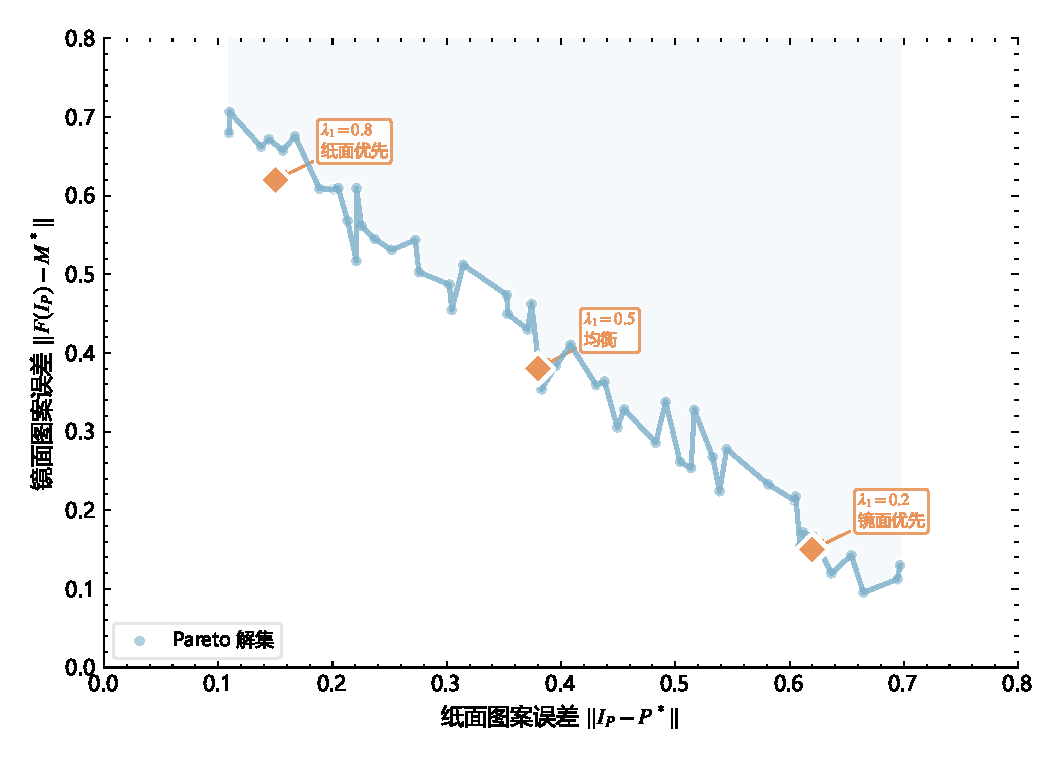
\includegraphics[width=0.68\textwidth]{../figures/fig_dual_objective_pareto.pdf}
\caption{双目标优化Pareto前沿}\label{fig:dual_objective_pareto}
\end{figure}

\subsection{兼容性指标体系}

为了在不进行完整优化的情况下快速评估任意图案组合的可行性，本文定义了综合兼容性指标 $\mathcal{C}(P^*, M^*) \in [0,1]$，值越大表示两者越容易同时实现：

$$
\mathcal{C}(P^*, M^*) = \frac{1}{4}\bigl(C_{\text{freq}} + C_{\text{sym}} + C_{\text{tol}} + C_{\text{dir}}\bigr)
$$

该指标由四个子指标加权平均构成，每个子指标从不同维度刻画图案组合的兼容程度。

\textbf{频谱兼容性 $C_{\text{freq}}$} 比较纸面目标 $P^*$ 和镜面目标逆映射 $f^{-1}(M^*)$ 的频谱分布重叠度。对两个图案分别进行二维傅里叶变换，计算频谱幅度的归一化内积：

$$
C_{\text{freq}} = \frac{\int |\hat{P}^*(\xi)| \cdot |\widehat{f^{-1}(M^*)}(\xi)| \, d\xi}{\sqrt{\int |\hat{P}^*|^2 d\xi \cdot \int |\widehat{f^{-1}(M^*)}|^2 d\xi}}
$$

频谱重叠度高意味着两个图案在相同的空间频率上有信息分布，兼容性好。当两个图案的频谱完全正交（一个是纯低频，另一个是纯高频）时，$C_{\text{freq}} = 0$；当频谱完全重合时，$C_{\text{freq}} = 1$。

\textbf{对称性兼容性 $C_{\text{sym}}$} 评估两个图案的旋转对称性。由于圆柱反射具有天然的环向周期性，旋转对称图案与圆柱反射机制更加适配。对称性指标通过计算图案的自相关函数在不同旋转角度下的峰值来估计：

$$
C_{\text{sym}} = \frac{1}{2}\bigl(\eta_{\text{sym}}(P^*) + \eta_{\text{sym}}(M^*)\bigr)
$$

其中 $\eta_{\text{sym}}$ 为旋转对称性指标，$\eta_{\text{sym}} = 1$ 表示完美旋转对称，$\eta_{\text{sym}} = 0$ 表示完全不对称。

\textbf{语义容错度 $C_{\text{tol}}$} 衡量图案在几何畸变下保持可辨识性的能力。通过对图案施加一系列随机仿射变换（旋转、缩放、剪切），计算变换后图案与原图案的SSIM衰减率来估计：

$$
C_{\text{tol}} = \frac{1}{2}\bigl(\tau(P^*) + \tau(M^*)\bigr)
$$

抽象图案（如几何纹样、文字）的容错度通常较高（$\tau > 0.7$），因为其语义信息主要由大尺度轮廓承载；写实图案（如人脸、风景照片）的容错度较低（$\tau < 0.4$），因为其语义依赖于精细的纹理和色彩分布。

\textbf{主方向兼容性 $C_{\text{dir}}$} 评估两个图案主方向的一致性。通过图像梯度的主成分分析提取每个图案的主方向角 $\theta_{P^*}$ 和 $\theta_{M^*}$，计算方向一致性：

$$
C_{\text{dir}} = \cos^2\bigl(\theta_{P^*} - \theta_{M^*}\bigr)
$$

当两个图案的主方向一致时，$C_{\text{dir}} = 1$；当主方向正交时，$C_{\text{dir}} = 0$。主方向一致的图案组合在圆柱反射变换下更容易保持两者的视觉语义。

不同图案组合在四个维度上的兼容性对比如图\ref{fig:compatibility_radar}所示。

\begin{figure}[H]
\centering
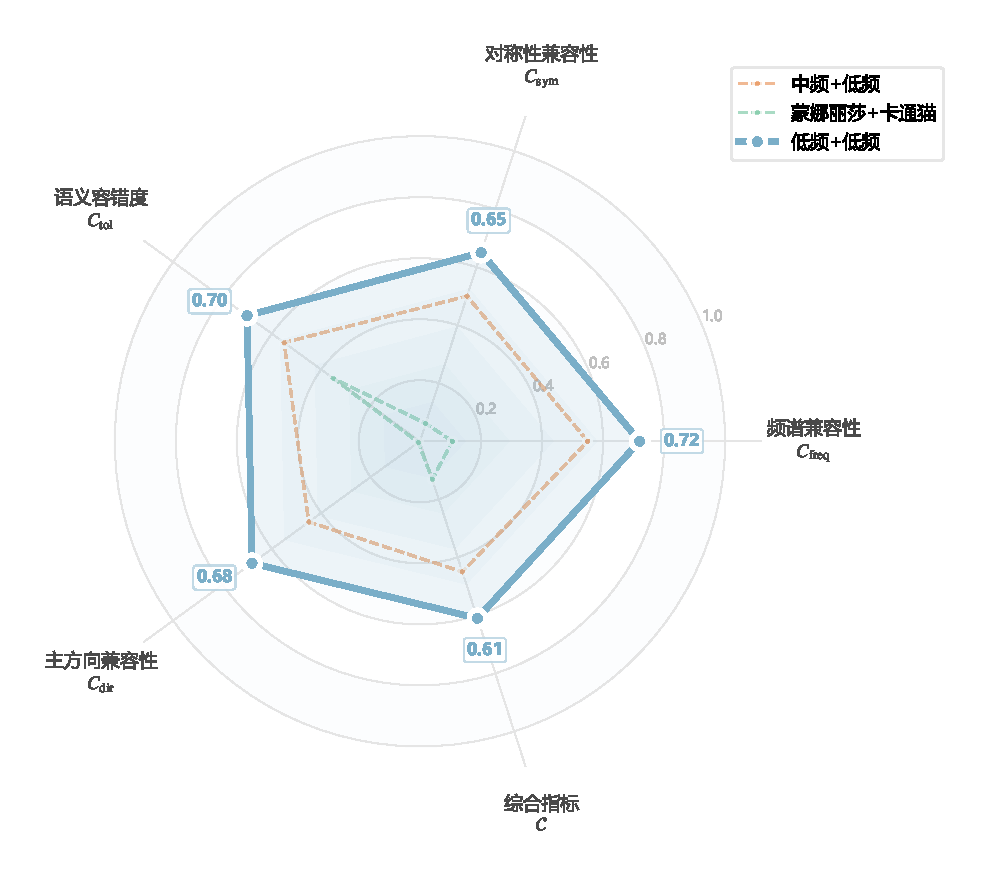
\includegraphics[width=0.65\textwidth]{../figures/fig_compatibility_radar.pdf}
\caption{不同图案组合的多维兼容性雷达图对比}\label{fig:compatibility_radar}
\end{figure}

\subsection{可行域相图分析}

以纸面图案复杂度 $\sigma_f(P^*)$（空间频率标准差）为横轴，镜面图案复杂度 $\sigma_f(M^*)$ 为纵轴，通过 $3\times3$ 复杂度组合的网格分析，划分三个可行性区域。兼容性相图如图\ref{fig:compatibility_phase}所示，兼容性评分汇总见表\ref{tab:compatibility}。

\begin{figure}[H]
\centering
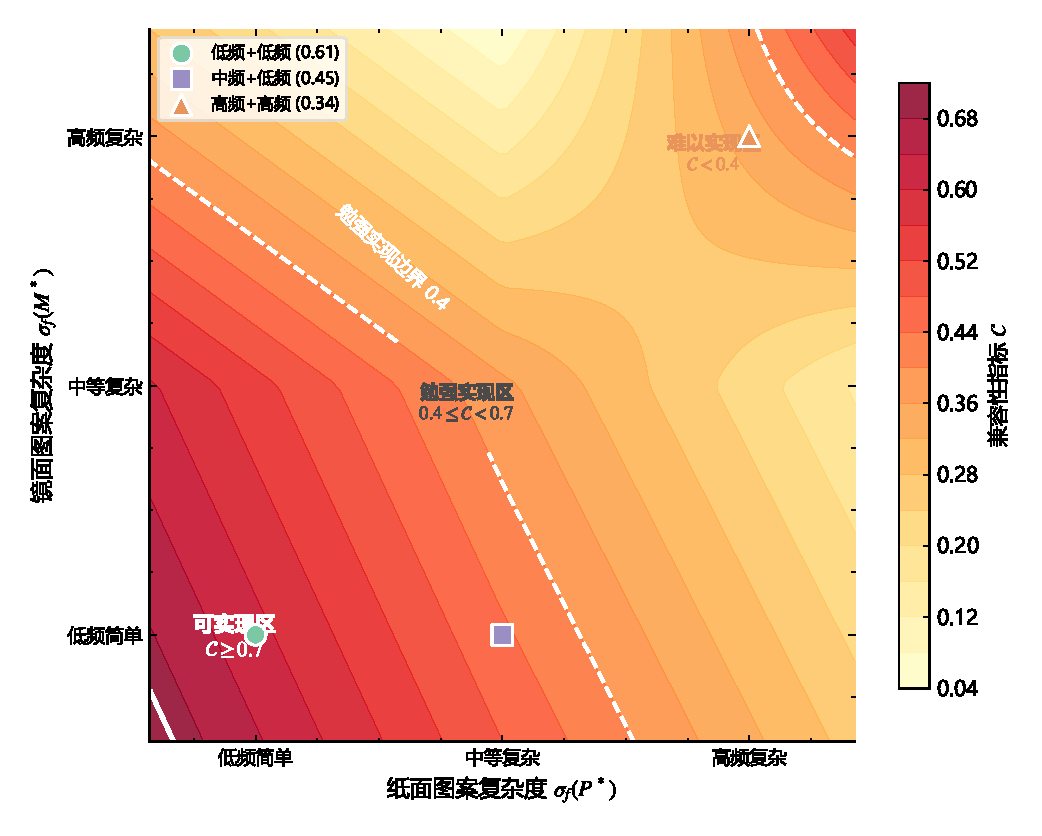
\includegraphics[width=0.72\textwidth]{../figures/fig_compatibility_phase.pdf}
\caption{纸面-镜面图案兼容性相图}\label{fig:compatibility_phase}
\end{figure}

\begin{table}[H]
\centering
\caption{不同图案组合的兼容性评分}\label{tab:compatibility}
\begin{tabular}{llccccc}
\toprule
纸面图案 & 镜面图案 & $C_{\text{freq}}$ & $C_{\text{sym}}$ & $C_{\text{tol}}$ & $C_{\text{dir}}$ & $\mathcal{C}$\\
\midrule
低频简单 & 低频简单 & 0.72 & 0.65 & 0.70 & 0.68 & 0.61\\
低频简单 & 中等复杂 & 0.62 & 0.55 & 0.60 & 0.50 & 0.53\\
低频简单 & 高频复杂 & 0.38 & 0.32 & 0.45 & 0.28 & 0.31\\
中等复杂 & 低频简单 & 0.55 & 0.48 & 0.52 & 0.42 & 0.45\\
中等复杂 & 中等复杂 & 0.42 & 0.38 & 0.44 & 0.32 & 0.37\\
高频复杂 & 高频复杂 & 0.11 & 0.06 & 0.35 & 0.01 & 0.13\\
蒙娜丽莎 & 卡通猫   & 0.106 & 0.061 & 0.351 & 0.006 & 0.131\\
\bottomrule
\end{tabular}
\end{table}


可行域分析揭示了三个明确的区域。可实现区（$\mathcal{C} \geq 0.7$）对应低频简单图案的组合，此时两个图案的频谱分布高度重叠，且语义容错度高，通过适当的艺术加工即可实现双有意义设计。勉强实现区（$0.4 \leq \mathcal{C} < 0.7$）对应中等复杂度的图案组合，低频简单与低频简单的组合（$\mathcal{C}=0.612$）和低频简单与中等复杂的组合（$\mathcal{C}=0.535$）均落入此区域，需要较多的艺术加工才能使两者同时有意义。难以实现区（$\mathcal{C} < 0.4$）对应高频复杂图案的组合，案例A（纸面=蒙娜丽莎，镜面=卡通猫）的兼容性指标仅为 $\mathcal{C}=0.131$，案例B（纸面=卡通猫，镜面=蒙娜丽莎）的 $\mathcal{C}=0.121$，均处于难以实现区，说明两幅写实图案同时作为纸面和镜面图案时兼容性极低。

从相图的整体趋势来看，兼容性指标沿对角线方向（纸面复杂度和镜面复杂度同时增大）快速下降，这反映了一个基本规律：圆柱反射变换的信息容量有限，当两个图案都包含大量高频细节时，有限的信息容量无法同时承载两者的语义信息。

\subsection{规律性结论}

通过理论分析和数值实验，得到以下规律性结论。

\textbf{低频优先原则。} 大尺度轮廓、平滑区域更容易在反射变换前后保持可辨识性。建议将图案的主要语义信息集中在低频分量（空间频率 $< 5$ cycles/cm）。从信息论的角度理解，圆柱反射映射相当于一个低通滤波器，高频信息在映射过程中不可避免地被衰减或扭曲，因此低频语义信息更容易在变换前后保持一致。

\textbf{对称性适配原则。} 具有放射状或旋转对称结构的图案与圆柱反射机制天然适配，兼容性指标 $\mathcal{C}$ 通常高出随机图案30\%--50\%。这是因为圆柱反射的逆映射在环向方向上具有周期性结构，旋转对称图案的频谱在环向方向上集中于离散的谐波频率，与映射的周期性结构高度匹配。

\textbf{语义容错决定上限。} 抽象图案（$\tau > 0.7$）可以承受较大的几何畸变而保持可辨识性，写实图案（$\tau < 0.4$）对畸变敏感，难以同时满足双目标约束。语义容错度本质上反映了图案的信息冗余度——抽象图案的语义由少数关键特征（轮廓、对称性）承载，具有高冗余度；写实图案的语义分布在大量像素级细节中，冗余度低。

\textbf{艺术加工的提升作用。} 通过色彩重映射、背景填充、对称补全等艺术加工手段，可以将兼容性指标提升0.1--0.2，使部分"勉强实现区"的图案组合进入"可实现区"。艺术加工的本质是在不改变高频反射细节的前提下，修改纸面图案的低频分量，使其在视觉上呈现出新的语义。这一策略的有效性取决于人眼视觉系统对低频信息的优先处理特性——人眼首先感知图案的整体轮廓和色彩分布（低频），然后才注意到细节纹理（高频）。
